%% bare_jrnl.tex
%% V1.4b
%% 2015/08/26
%% by Michael Shell
%% see http://www.michaelshell.org/
%% for current contact information.
%%
%% This is a skeleton file demonstrating the use of IEEEtran.cls
%% (requires IEEEtran.cls version 1.8b or later) with an IEEE
%% journal paper.
%%
%% Support sites:
%% http://www.michaelshell.org/tex/ieeetran/
%% http://www.ctan.org/pkg/ieeetran
%% and
%% http://www.ieee.org/

%%*************************************************************************
%% Legal Notice:
%% This code is offered as-is without any warranty either expressed or
%% implied; without even the implied warranty of MERCHANTABILITY or
%% FITNESS FOR A PARTICULAR PURPOSE! 
%% User assumes all risk.
%% In no event shall the IEEE or any contributor to this code be liable for
%% any damages or losses, including, but not limited to, incidental,
%% consequential, or any other damages, resulting from the use or misuse
%% of any information contained here.
%%
%% All comments are the opinions of their respective authors and are not
%% necessarily endorsed by the IEEE.
%%
%% This work is distributed under the LaTeX Project Public License (LPPL)
%% ( http://www.latex-project.org/ ) version 1.3, and may be freely used,
%% distributed and modified. A copy of the LPPL, version 1.3, is included
%% in the base LaTeX documentation of all distributions of LaTeX released
%% 2003/12/01 or later.
%% Retain all contribution notices and credits.
%% ** Modified files should be clearly indicated as such, including  **
%% ** renaming them and changing author support contact information. **
%%*************************************************************************


% *** Authors should verify (and, if needed, correct) their LaTeX system  ***
% *** with the testflow diagnostic prior to trusting their LaTeX platform ***
% *** with production work. The IEEE's font choices and paper sizes can   ***
% *** trigger bugs that do not appear when using other class files.       ***                          ***
% The testflow support page is at:
% http://www.michaelshell.org/tex/testflow/
\usepackage{indentfirst}




\documentclass[journal]{IEEEtran}
%
% If IEEEtran.cls has not been installed into the LaTeX system files,
% manually specify the path to it like:
% \documentclass[journal]{../sty/IEEEtran}





% Some very useful LaTeX packages include:
% (uncomment the ones you want to load)


% *** MISC UTILITY PACKAGES ***
%
%\usepackage{ifpdf}
% Heiko Oberdiek's ifpdf.sty is very useful if you need conditional
% compilation based on whether the output is pdf or dvi.
% usage:
% \ifpdf
%   % pdf code
% \else
%   % dvi code
% \fi
% The latest version of ifpdf.sty can be obtained from:
% http://www.ctan.org/pkg/ifpdf
% Also, note that IEEEtran.cls V1.7 and later provides a builtin
% \ifCLASSINFOpdf conditional that works the same way.
% When switching from latex to pdflatex and vice-versa, the compiler may
% have to be run twice to clear warning/error messages.






% *** CITATION PACKAGES ***
%
%\usepackage{cite}
% cite.sty was written by Donald Arseneau
% V1.6 and later of IEEEtran pre-defines the format of the cite.sty package
% \cite{} output to follow that of the IEEE. Loading the cite package will
% result in citation numbers being automatically sorted and properly
% "compressed/ranged". e.g., [1], [9], [2], [7], [5], [6] without using
% cite.sty will become [1], [2], [5]--[7], [9] using cite.sty. cite.sty's
% \cite will automatically add leading space, if needed. Use cite.sty's
% noadjust option (cite.sty V3.8 and later) if you want to turn this off
% such as if a citation ever needs to be enclosed in parenthesis.
% cite.sty is already installed on most LaTeX systems. Be sure and use
% version 5.0 (2009-03-20) and later if using hyperref.sty.
% The latest version can be obtained at:
% http://www.ctan.org/pkg/cite
% The documentation is contained in the cite.sty file itself.






% *** GRAPHICS RELATED PACKAGES ***
%
\ifCLASSINFOpdf
   \usepackage[pdftex]{graphicx}
%   declare the path(s) where your graphic files are
   \graphicspath{{../pdf/}{../jpeg/}}
%   and their extensions so you won't have to specify these with
%   every instance of \includegraphics
   \DeclareGraphicsExtensions{.pdf,.jpeg,.png}
\else
%   or other class option (dvipsone, dvipdf, if not using dvips). graphicx
%   will default to the driver specified in the system graphics.cfg if no
%   driver is specified.
   \usepackage[dvips]{graphicx}
%   declare the path(s) where your graphic files are
   \graphicspath{{../eps/}}
%   and their extensions so you won't have to specify these with
%   every instance of \includegraphics
   \DeclareGraphicsExtensions{.eps}
\fi
% graphicx was written by David Carlisle and Sebastian Rahtz. It is
% required if you want graphics, photos, etc. graphicx.sty is already
% installed on most LaTeX systems. The latest version and documentation
% can be obtained at: 
% http://www.ctan.org/pkg/graphicx
% Another good source of documentation is "Using Imported Graphics in
% LaTeX2e" by Keith Reckdahl which can be found at:
% http://www.ctan.org/pkg/epslatex
%
% latex, and pdflatex in dvi mode, support graphics in encapsulated
% postscript (.eps) format. pdflatex in pdf mode supports graphics
% in .pdf, .jpeg, .png and .mps (metapost) formats. Users should ensure
% that all non-photo figures use a vector format (.eps, .pdf, .mps) and
% not a bitmapped formats (.jpeg, .png). The IEEE frowns on bitmapped formats
% which can result in "jaggedy"/blurry rendering of lines and letters as
% well as large increases in file sizes.
%
% You can find documentation about the pdfTeX application at:
% http://www.tug.org/applications/pdftex





% *** MATH PACKAGES ***
%
%\usepackage{amsmath}
% A popular package from the American Mathematical Society that provides
% many useful and powerful commands for dealing with mathematics.
%
% Note that the amsmath package sets \interdisplaylinepenalty to 10000
% thus preventing page breaks from occurring within multiline equations. Use:
%\interdisplaylinepenalty=2500
% after loading amsmath to restore such page breaks as IEEEtran.cls normally
% does. amsmath.sty is already installed on most LaTeX systems. The latest
% version and documentation can be obtained at:
% http://www.ctan.org/pkg/amsmath





% *** SPECIALIZED LIST PACKAGES ***
%
\usepackage{algorithmic}
\usepackage{algorithmicx}
\usepackage{algpseudocode}
\usepackage{algorithm}
% algorithmic.sty was written by Peter Williams and Rogerio Brito.
% This package provides an algorithmic environment fo describing algorithms.
% You can use the algorithmic environment in-text or within a figure
% environment to provide for a floating algorithm. Do NOT use the algorithm
% floating environment provided by algorithm.sty (by the same authors) or
% algorithm2e.sty (by Christophe Fiorio) as the IEEE does not use dedicated
% algorithm float types and packages that provide these will not provide
% correct IEEE style captions. The latest version and documentation of
% algorithmic.sty can be obtained at:
% http://www.ctan.org/pkg/algorithms
% Also of interest may be the (relatively newer and more customizable)
% algorithmicx.sty package by Szasz Janos:
% http://www.ctan.org/pkg/algorithmicx




% *** ALIGNMENT PACKAGES ***
%
%\usepackage{array}
% Frank Mittelbach's and David Carlisle's array.sty patches and improves
% the standard LaTeX2e array and tabular environments to provide better
% appearance and additional user controls. As the default LaTeX2e table
% generation code is lacking to the point of almost being broken with
% respect to the quality of the end results, all users are strongly
% advised to use an enhanced (at the very least that provided by array.sty)
% set of table tools. array.sty is already installed on most systems. The
% latest version and documentation can be obtained at:
% http://www.ctan.org/pkg/array


% IEEEtran contains the IEEEeqnarray family of commands that can be used to
% generate multiline equations as well as matrices, tables, etc., of high
% quality.




% *** SUBFIGURE PACKAGES ***
\ifCLASSOPTIONcompsoc
 \usepackage[caption=false,font=normalsize,labelfont=sf,textfont=sf]{subfig}
\else
 \usepackage[caption=false,font=footnotesize]{subfig}
\fi
% subfig.sty, written by Steven Douglas Cochran, is the modern replacement
% for subfigure.sty, the latter of which is no longer maintained and is
% incompatible with some LaTeX packages including fixltx2e. However,
% subfig.sty requires and automatically loads Axel Sommerfeldt's caption.sty
% which will override IEEEtran.cls' handling of captions and this will result
% in non-IEEE style figure/table captions. To prevent this problem, be sure
% and invoke subfig.sty's "caption=false" package option (available since
% subfig.sty version 1.3, 2005/06/28) as this is will preserve IEEEtran.cls
% handling of captions.
% Note that the Computer Society format requires a larger sans serif font
% than the serif footnote size font used in traditional IEEE formatting
% and thus the need to invoke different subfig.sty package options depending
% on whether compsoc mode has been enabled.
%
% The latest version and documentation of subfig.sty can be obtained at:
% http://www.ctan.org/pkg/subfig




% *** FLOAT PACKAGES ***
%
%\usepackage{fixltx2e}
% fixltx2e, the successor to the earlier fix2col.sty, was written by
% Frank Mittelbach and David Carlisle. This package corrects a few problems
% in the LaTeX2e kernel, the most notable of which is that in current
% LaTeX2e releases, the ordering of single and double column floats is not
% guaranteed to be preserved. Thus, an unpatched LaTeX2e can allow a
% single column figure to be placed prior to an earlier double column
% figure.
% Be aware that LaTeX2e kernels dated 2015 and later have fixltx2e.sty's
% corrections already built into the system in which case a warning will
% be issued if an attempt is made to load fixltx2e.sty as it is no longer
% needed.
% The latest version and documentation can be found at:
% http://www.ctan.org/pkg/fixltx2e


%\usepackage{stfloats}
% stfloats.sty was written by Sigitas Tolusis. This package gives LaTeX2e
% the ability to do double column floats at the bottom of the page as well
% as the top. (e.g., "\begin{figure*}[!b]" is not normally possible in
% LaTeX2e). It also provides a command:
%\fnbelowfloat
% to enable the placement of footnotes below bottom floats (the standard
% LaTeX2e kernel puts them above bottom floats). This is an invasive package
% which rewrites many portions of the LaTeX2e float routines. It may not work
% with other packages that modify the LaTeX2e float routines. The latest
% version and documentation can be obtained at:
% http://www.ctan.org/pkg/stfloats
% Do not use the stfloats baselinefloat ability as the IEEE does not allow
% \baselineskip to stretch. Authors submitting work to the IEEE should note
% that the IEEE rarely uses double column equations and that authors should try
% to avoid such use. Do not be tempted to use the cuted.sty or midfloat.sty
% packages (also by Sigitas Tolusis) as the IEEE does not format its papers in
% such ways.
% Do not attempt to use stfloats with fixltx2e as they are incompatible.
% Instead, use Morten Hogholm'a dblfloatfix which combines the features
% of both fixltx2e and stfloats:
%
% \usepackage{dblfloatfix}
% The latest version can be found at:
% http://www.ctan.org/pkg/dblfloatfix




%\ifCLASSOPTIONcaptionsoff
%  \usepackage[nomarkers]{endfloat}
% \let\MYoriglatexcaption\caption
% \renewcommand{\caption}[2][\relax]{\MYoriglatexcaption[#2]{#2}}
%\fi
% endfloat.sty was written by James Darrell McCauley, Jeff Goldberg and 
% Axel Sommerfeldt. This package may be useful when used in conjunction with 
% IEEEtran.cls'  captionsoff option. Some IEEE journals/societies require that
% submissions have lists of figures/tables at the end of the paper and that
% figures/tables without any captions are placed on a page by themselves at
% the end of the document. If needed, the draftcls IEEEtran class option or
% \CLASSINPUTbaselinestretch interface can be used to increase the line
% spacing as well. Be sure and use the nomarkers option of endfloat to
% prevent endfloat from "marking" where the figures would have been placed
% in the text. The two hack lines of code above are a slight modification of
% that suggested by in the endfloat docs (section 8.4.1) to ensure that
% the full captions always appear in the list of figures/tables - even if
% the user used the short optional argument of \caption[]{}.
% IEEE papers do not typically make use of \caption[]'s optional argument,
% so this should not be an issue. A similar trick can be used to disable
% captions of packages such as subfig.sty that lack options to turn off
% the subcaptions:
% For subfig.sty:
% \let\MYorigsubfloat\subfloat
% \renewcommand{\subfloat}[2][\relax]{\MYorigsubfloat[]{#2}}
% However, the above trick will not work if both optional arguments of
% the \subfloat command are used. Furthermore, there needs to be a
% description of each subfigure *somewhere* and endfloat does not add
% subfigure captions to its list of figures. Thus, the best approach is to
% avoid the use of subfigure captions (many IEEE journals avoid them anyway)
% and instead reference/explain all the subfigures within the main caption.
% The latest version of endfloat.sty and its documentation can obtained at:
% http://www.ctan.org/pkg/endfloat
%
% The IEEEtran \ifCLASSOPTIONcaptionsoff conditional can also be used
% later in the document, say, to conditionally put the References on a 
% page by themselves.




% *** PDF, URL AND HYPERLINK PACKAGES ***
%
%\usepackage{url}
% url.sty was written by Donald Arseneau. It provides better support for
% handling and breaking URLs. url.sty is already installed on most LaTeX
% systems. The latest version and documentation can be obtained at:
% http://www.ctan.org/pkg/url
% Basically, \url{my_url_here}.




% *** Do not adjust lengths that control margins, column widths, etc. ***
% *** Do not use packages that alter fonts (such as pslatex).         ***
% There should be no need to do such things with IEEEtran.cls V1.6 and later.
% (Unless specifically asked to do so by the journal or conference you plan
% to submit to, of course. )


% correct bad hyphenation here
\hyphenation{op-tical net-works semi-conduc-tor}


\begin{document}
%
% paper title
% Titles are generally capitalized except for words such as a, an, and, as,
% at, but, by, for, in, nor, of, on, or, the, to and up, which are usually
% not capitalized unless they are the first or last word of the title.
% Linebreaks \\ can be used within to get better formatting as desired.
% Do not put math or special symbols in the title.


%%%%%%%%%%%%%%%%%%%%%%%%%%%%%%%%%%%%%%%%%%%%%% TITLE %%%%%%%%%%%%%%%%%%%%%%%%%%%%%%%%%%%%%%%%%%%%%%%%%%%%%%%%%%%%%%%%%

%\title{Bare Demo of IEEEtran.cls\\ for IEEE Journals}
\title{Benchmarking Spiking Neural Networks\\ with Multiprocessing}
%
%
% author names and IEEE memberships
% note positions of commas and nonbreaking spaces ( ~ ) LaTeX will not break
% a structure at a ~ so this keeps an author's name from being broken across
% two lines.
% use \thanks{} to gain access to the first footnote area
% a separate \thanks must be used for each paragraph as LaTeX2e's \thanks
% was not built to handle multiple paragraphs
%

\author{Isaac~Bettendorf,~\IEEEmembership{Student,~Virgina Tech,}
        Osaze~Shears,~\IEEEmembership{Student,~Virginia Tech}
        % and~Jane~Doe,~\IEEEmembership{Life~Fellow,~IEEE}% <-this % stops a space
% \thanks{M. Shell was with the Department
% of Electrical and Computer Engineering, Georgia Institute of Technology, Atlanta,
% GA, 30332 USA e-mail: (see http://www.michaelshell.org/contact.html).}% <-this % stops a space
% \thanks{J. Doe and J. Doe are with Anonymous University.}% <-this % stops a space
% \thanks{Manuscript received April 19, 2005; revised August 26, 2015.}}
}



%%%%%%%%%%%%%%%%%%%%%%%%%%%%%%%%%%%%%%%%%%%%%%%%%%%%%%%%%%%%%%%%%%%%%%%%%%%%%%%%%%%%%%%%%%%%%%%%%%%%%%%%%%%%%%%%%%%%%%%%%%



% note the % following the last \IEEEmembership and also \thanks - 
% these prevent an unwanted space from occurring between the last author name
% and the end of the author line. i.e., if you had this:
% 
% \author{....lastname \thanks{...} \thanks{...} }
%                     ^------------^------------^----Do not want these spaces!
%
% a space would be appended to the last name and could cause every name on that
% line to be shifted left slightly. This is one of those "LaTeX things". For
% instance, "\textbf{A} \textbf{B}" will typeset as "A B" not "AB". To get
% "AB" then you have to do: "\textbf{A}\textbf{B}"
% \thanks is no different in this regard, so shield the last } of each \thanks
% that ends a line with a % and do not let a space in before the next \thanks.
% Spaces after \IEEEmembership other than the last one are OK (and needed) as
% you are supposed to have spaces between the names. For what it is worth,
% this is a minor point as most people would not even notice if the said evil
% space somehow managed to creep in.



% The paper headers
\markboth{VT ECE5510 Class Final Project, December~2020}%
{Shell \MakeLowercase{\textit{et al.}}: Bare Demo of IEEEtran.cls for IEEE Journals}
% The only time the second header will appear is for the odd numbered pages
% after the title page when using the twoside option.
% 
% *** Note that you probably will NOT want to include the author's ***
% *** name in the headers of peer review papers.                   ***
% You can use \ifCLASSOPTIONpeerreview for conditional compilation here if
% you desire.



% If you want to put a publisher's ID mark on the page you can do it like
% this:
%\IEEEpubid{0000--0000/00\$00.00~\copyright~2015 IEEE}
% Remember, if you use this you must call \IEEEpubidadjcol in the second
% column for its text to clear the IEEEpubid mark.



% use for special paper notices
%\IEEEspecialpapernotice{(Invited Paper)}




% make the title area
\maketitle

% As a general rule, do not put math, special symbols or citations
% in the abstract or keywords.

%%%%%%%%%%%%%%%%%%%%%%%%%%%%%% ABSTRACT ABSTRACT ABSTRACT %%%%%%%%%%%%%%%%%%%%%%%%%%%%%%%%%%%%%%%%%%%%%%%%%%%%%%%%

\begin{abstract}
The abstract goes here.
\end{abstract}

% Note that keywords are not normally used for peerreview papers.
\begin{IEEEkeywords}
multiprocessing, spiking neural networks, neuromorphic computing, graphics processing unit, CUDA
\end{IEEEkeywords}

%%%%%%%%%%%%%%%%%%%%%%%%%%%%%%%%%%%%%%%%%%%%%%%%%%%%%%%%%%%%%%%%%%%%%%%%%%%%%%%%%%%%%%%%%%%%%%%%%%%%%%%%%%%%%%%%%%




% For peer review papers, you can put extra information on the cover
% page as needed:
% \ifCLASSOPTIONpeerreview
% \begin{center} \bfseries EDICS Category: 3-BBND \end{center}
% \fi
%
% For peerreview papers, this IEEEtran command inserts a page break and
% creates the second title. It will be ignored for other modes.
\IEEEpeerreviewmaketitle

%%%%%%%%%%%%%%%%%%%%%%%%%%%%%%%%%%%%%%%% BODY OF PAPER %%%%%%%%%%%%%%%%%%%%%%%%%%%%%%%%%%%%%%%%%%%%%%%%%%%%%%%%%%%%%%%%%%%

\section{INTRODUCTION}
% The very first letter is a 2 line initial drop letter followed
% by the rest of the first word in caps.
% 
% form to use if the first word consists of a single letter:
% \IEEEPARstart{A}{demo} file is ....
% 
% form to use if you need the single drop letter followed by
% normal text (unknown if ever used by the IEEE):
% \IEEEPARstart{A}{}demo file is ....
% 
% Some journals put the first two words in caps:
% \IEEEPARstart{T}{his demo} file is ....
% 
% Here we have the typical use of a "T" for an initial drop letter
% and "HIS" in caps to complete the first word.

\IEEEPARstart{T}{he} brain is a massively asynchronous and parallel computational machine \cite{zeki2015massively,hawkins2004intelligence,shanahan2015technological}. While modern computers become increasingly faster at performing tasks that are easily accomplished with sequential arithmetic and logic operations, they still fall short in performing tasks such as image recognition and abstract thinking with the speed and power efficiency of the human brain \cite{hawkins2004intelligence,shanahan2015technological}. 

\subsection{Evolution of Modern Computer Architecture}

Modern computer architecture evolved from the Von Neumann architecture and their designs have carried with them a bottleneck in the system bus which makes a multiprocessor design very unscalable. One method to increase throughput despite this shortcoming is to utilize specialized processing hardware such as graphic processing units (GPU). A GPU is composed of many specialized arithmetic processing units (ALU) for matrix multiplication and can typically perform hundreds of such calculations simultaneously.

\subsection{Artificial Neural Networks}

Artificial neural networks (ANN) are a group of algorithms designed to mimic the behavior of biological neural networks seen in the brain with nodes or neuron models and their connections being the ANN's most basic elements. These ANN are formed by training. During training, inputs, whose expected outputs are known, are fed into the ANN. These inputs then propagate through the system producing outputs which may or may not be correct. This process is known as \emph{forward propagation}. The ANN then performs a process known as \emph{back propagation} in which parameters of this network are adjusted compensating for the difference between the actual output and the desired output. Traditionally in ANN, it is the forward propagation which utilizes matrix multiplication and can potentially use GPU to speedup this part of the training process. More specialized neuromorphic hardware exists where each neuron model is represented in hardware. Where neuromorphic hardware is more scalable for power and integrated circuit (IC) real estate compared to the GPU, both suffer from the unscalability of multiplier circuits [ , ].

\subsection{Spiking Neural Networks}

Spiking neural networks (SNN) are a form of ANN that more closely simulate natural neural networks. They are inherently asynchronous because SNNs do not have optimizers like traditional ANN. Optimization in ANNs traditionally needs to be synchronous, meaning how one node optimizes affects the other nodes' optimization. To contrast, SNN nodes simply wait to receive spikes from other nodes within a simulation time step. The state of one node is not necessarily dependent on the state of all nodes at a given instance. A node in a SNN is only focused on the nodes whose connections are coming into it. However, there is a synchronous aspect to SNNs in that a node must wait to continue operating until all nodes have reached the end of the time step\cite{Bouvier2019}.

\par

SNN are massively parallel because of the asynchronous nature of each node. In each layer, a node can potentially be simulated in its own thread. In this article's implementation of a multithreaded SNN, there are groups of nodes (of the same layer) being simulated by a single thread; however, studying the performance on this architecture may provide insight for the development of future architectures. 

\subsection{Article Organization}

This article, inspired by the work seen in \cite{ma2019stochastic}, studies the performance of SNN on distributed or non-uniform memory access (NUMA) architecture as opposed to the more traditional Von Neumann uniform memory access (UMA) architecture. First, this article 
% You must have at least 2 lines in the paragraph with the drop letter
% (should never be an issue)

%\hfill mds
 
%\hfill August 26, 2015

%%%%%%%%%%%%\subsection{Subsection Heading Here}
%%%%%%%%%%%%Subsection text here.

% needed in second column of first page if using \IEEEpubid
%\IEEEpubidadjcol

%%%%%%%%%%%%\subsubsection{Subsubsection Heading Here}
%%%%%%%%%%%%Subsubsection text here.


% An example of a floating figure using the graphicx package.
% Note that \label must occur AFTER (or within) \caption.
% For figures, \caption should occur after the \includegraphics.
% Note that IEEEtran v1.7 and later has special internal code that
% is designed to preserve the operation of \label within \caption
% even when the captionsoff option is in effect. However, because
% of issues like this, it may be the safest practice to put all your
% \label just after \caption rather than within \caption{}.
%
% Reminder: the "draftcls" or "draftclsnofoot", not "draft", class
% option should be used if it is desired that the figures are to be
% displayed while in draft mode.

% \begin{figure}[!t]
% \centering
% \includegraphics[width=2.5in]{myfigure}
% where an .eps filename suffix will be assumed under latex, 
% and a .pdf suffix will be assumed for pdflatex; or what has been declared
% via \DeclareGraphicsExtensions.
% \caption{Simulation results for the network.}
% \label{fig_sim}
% \end{figure}

% Note that the IEEE typically puts floats only at the top, even when this
% results in a large percentage of a column being occupied by floats.


% An example of a double column floating figure using two subfigures.
% (The subfig.sty package must be loaded for this to work.)
% The subfigure \label commands are set within each subfloat command,
% and the \label for the overall figure must come after \caption.
% \hfil is used as a separator to get equal spacing.
% Watch out that the combined width of all the subfigures on a 
% line do not exceed the text width or a line break will occur.
%
%\begin{figure*}[!t]
%\centering
%\subfloat[Case I]{\includegraphics[width=2.5in]{box}%
%\label{fig_first_case}}
%\hfil
%\subfloat[Case II]{\includegraphics[width=2.5in]{box}%
%\label{fig_second_case}}
%\caption{Simulation results for the network.}
%\label{fig_sim}
%\end{figure*}
%
% Note that often IEEE papers with subfigures do not employ subfigure
% captions (using the optional argument to \subfloat[]), but instead will
% reference/describe all of them (a), (b), etc., within the main caption.
% Be aware that for subfig.sty to generate the (a), (b), etc., subfigure
% labels, the optional argument to \subfloat must be present. If a
% subcaption is not desired, just leave its contents blank,
% e.g., \subfloat[].


% An example of a floating table. Note that, for IEEE style tables, the
% \caption command should come BEFORE the table and, given that table
% captions serve much like titles, are usually capitalized except for words
% such as a, an, and, as, at, but, by, for, in, nor, of, on, or, the, to
% and up, which are usually not capitalized unless they are the first or
% last word of the caption. Table text will default to \footnotesize as
% the IEEE normally uses this smaller font for tables.
% The \label must come after \caption as always.
%
% \begin{table}[!t]
% %% increase table row spacing, adjust to taste
% \renewcommand{\arraystretch}{1.3}
% % if using array.sty, it might be a good idea to tweak the value of
% % \extrarowheight as needed to properly center the text within the cells
% %\caption{An Example of a Table}
% \label{table_example}
% \centering
% %% Some packages, such as MDW tools, offer better commands for making tables
% %% than the plain LaTeX2e tabular which is used here.
% \begin{tabular}{|c||c|}
% \hline
% One & Two\\
% \hline
% Three & Four\\
% \hline
% \end{tabular}
% \end{table}

\section{Background}

\subsection{Spiking Neural Network Mechanics}

Spiking neural networks (SNNs) are fundamentally from ANNs because their operation occurs over a period of time. At each time step the neurons in an SNN receive weighted spikes that either increment or decrements the neuron's membrane potential. Once the membrane potential of a neuron exceeds a predetermined threshold value, the neuron itself emits a spike. After emitting a spike, the neuron resets its membrane potential to its initial value and stops its membrane potential from changing for a period of time called the "refractory period".

There are three components that are needed to simulate an SNN:

\begin{itemize}
\item an encoding scheme
\item a neuron model
\item a learning rule
\end{itemize}

\subsubsection{Encoding Schemes}

Encoding schemes are necessary to specify the way that numerical input data is converted into spikes that occur over time. Typically each feature of the input data is mapped to an input neuron that generates spikes for the rest of the SNN. Our project looks at two different styles of encoding data: rate coding and temporal coding.

\begin{figure}[!t]
\centering
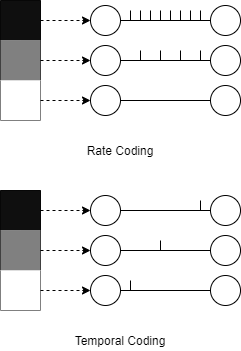
\includegraphics[width=1.75in]{encodings.png}
\caption{Spiking Neural Network Encoding Schemes}
\label{fig_sim}
\end{figure}

\textbf{Rate coding} works by adjusting the rate at which input neurons fire based on the intensity of the input data. Input neurons mapped to higher intensities fire more frequently, while input neurons mapped to lower intensities fire less. In several studies, the firing rate is also determined using a Poisson distribution, where higher intensity input neurons are more likely to fire. While rate coding is a noise-resistant way to represent data, it causes the network to consume more power when implemented in hardware.

\textbf{Temporal coding} works by adjusting the time at which input neurons fire based on the intensity of the input data. Input neurons mapped to higher intensities fire earlier compared to inputs with lower intensities. Rank order coding is one example of temporal coding where the input neurons fire in a discrete order determined by their intensities. Temporal coding is more power efficient than rate coding because of its sparsity, however, it is very susceptible to noise \cite{thorpe1998rank}.

A visual representation of the behaviors of these two encoding schemes is shown in \textbf{Figure 1}.


% LIF Model
\subsubsection{Neuron Models}

Another component required for simulating SNNs is the neuron model. Similar to the activation function in an ANN, the neuron model uses the inputs provided at the synapses to determine the output value of the neuron. The primary difference between the two is that a neuron model in an SNN will not provide any output if its membrane potential has not reached a certain threshold.

\begin{figure}[!t]
\centering
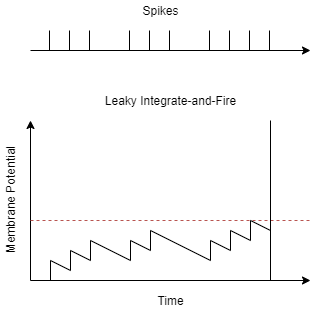
\includegraphics[width=2.5in]{lif_model.png}
\caption{Leaky Integrate-and-Fire (LIF) Neuron Model}
\label{fig_sim}
\end{figure}

In our project, we conducted experiments using the \textbf{leaky integrate-and-fire (LIF)} neuron model. In this model, weighted spikes that arrive at the neuron increase the membrane potential normally. However, at each timestep, the membrane potential constantly decays towards a resting value. This behavior prevents neurons that are not frequently stimulated from firing \cite{burkitt2006review}.

A visual representation of the behaviors of this neuron model is shown in \textbf{Figure 2}.

% 
\subsubsection{Spike-Timing Dependent Plasticity}

\textbf{Spike-timing dependent plasticity (STDP)} is a common unsupervised learning rule used to train SNNs. In this learning technique, the influence that a pre-synaptic neuron has on a post-synaptic neuron is adjusted based on the time elapsed between their emitted spikes. As shown in \textbf{Figure 3}, if a pre-synaptic neuron (i) fires just before a post-synaptic neuron (j), then the weight of the synapse connecting those two neurons is incremented (i.e., the pre-synaptic neuron firing had a strong correlation to the post-synaptic neuron firing). Alternatively, if a pre-synaptic neuron (i) fires just after a post-synaptic neuron (j), then the weight between those two neurons is decremented (i.e., the pre-synaptic neuron firing had no correlation to the post-synaptic neuron firing) \cite{Sjostrom:2010}. STDP is an inherently asynchronous algorithm since each synapse performs its weight updates independently from the other synapses.

\begin{figure}[!t]
\centering
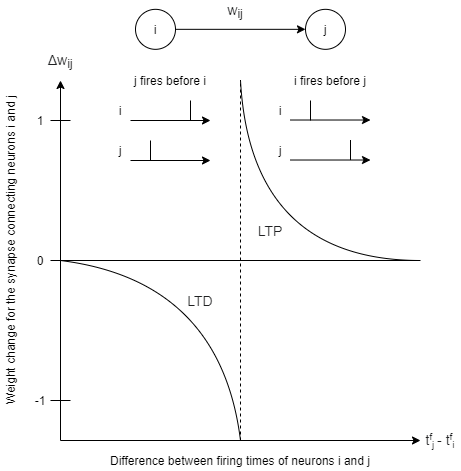
\includegraphics[width=2.5in]{stdp.png}
\caption{Leaky Integrate-and-Fire (LIF) Neuron Model}
\label{fig_sim}
\end{figure}

\subsection{Convolutional Neural Network}
Convolutional neural networks (CNN) are traditional ANNs with the added functionality given by specialized layers with the most important of these special layers being the convolutional whose function is to learn and form filters that best assist in the classification process.

\subsection{Computer Architecture}
This article presents the two main architectures used in this work. The first is Virginia Tech's RLogin which is a NUMA based architecture consisting of 64 Intel Xeon(R) Gold 5218 (at 2.30GHz) CPUs. Virginia Tech's GPU cluster was composed of one Nvidia Tesla T4 (rev a1) GPU and eight Intel Xeon(R) E5-2630 v3 (at 2.40 GHz) CPUs. CNNs that are composed of 2 dimensional convolutional layers are ideal for image processing.

\begin{table}[hbt!]
\caption {Hardware Specifications} \label{tab:title}
%% increase table row spacing, adjust to taste
\renewcommand{\arraystretch}{1.3}
% if using array.sty, it might be a good idea to tweak the value of
% \extrarowheight as needed to properly center the text within the cells
%\caption{An Example of a Table}
\label{Architecture_Table}
\centering
%% Some packages, such as MDW tools, offer better commands for making tables
%% than the plain LaTeX2e tabular which is used here.
\begin{tabular}{|c||c||c|}
\hline
\textbf{Element Name} & \textbf{CPU NUMA} & \textbf{GPU + CPU NUMA} \\
\hline
CPU/MP & 64 & 1 GPU + 8 CPU\\
\hline
Cores & 16 perCPU & 2560CUDA (totalGPU) + 8perCPU \\
\hline
Blocks & -- & 4 Per MP \\
\hline
Threads & 32 perCPU & 2560 \\
\hline
L1 (i+d) Cache & 32+32 KB & 32+32 KB (for CPU) \\
\hline
L2 Cache & 1024 KB & 4096 KB (for CPU) \\
\hline
L3 (shared) & 22528 KB & 16384 KB (for CPU) \\
\hline
RAM/global & 383 GB & 16 GB for GPU + 32 GB for CPU \\
\hline
\end{tabular}
%\caption{\label{tab:}Hardware Specifications}
\end{table}

TABLE 1 depicts the architecture's further specifications. Each NUMA node are connected by high-bandwidth interconnects and DRAM access on another node is transferred over the interconnects. This transfer takes longer than locally accessed memory. 
\par
The GPU is composed of multiple streaming multiprocessors (MP). Each MP is driven by the CUDA programming model. Thousands of threads can potentially run simultaneously on the GPU. But the work passed to the GPU is specialized and done so in a manner similar to passing a function from the CPU \cite{Gupta2020}. The passed information consists of a logical thread identifier that allows the different threads to work on different sections of the data \cite{Gupta2020}.

\subsection{Related Work}

\subsubsection{Stochastic Gradient Descent on Hardware}

In their research, Ma et al. (2019) benchmarked two different styles of multithreaded stochastic gradient descent (SGD) on both CPU and GPU hardware \cite{ma2019stochastic}. Their synchronous SGD algorithm allowed the threads to concurrently compute the gradient based on their training samples, and required the threads to synchronize after this calculation so that the main thread could perform the weight updates. Alternatively, their asynchronous SGD allowed the threads to both concurrently compute the gradient based on their training samples and update the weights accordingly.

The group found that when synchronous SGD was run using a GPU it sped up the training time by approximately 7X for deep neural networks compared to the CPU implementation. Additionally, asynchronous SGD performed on a multithreaded CPU outperformed the GPU version by more than 10X.

\subsubsection{BindsNET}

\subsubsection{Fast Spiking Neural Network Architecture for Low-cost FPGA Devices}
\par
The source \cite{iakymchuk2012fast} implements a SNN on a Xilinx Spartan 3 FPGA. Each neuron utilizes a Postsynaptic Potential (PSP) function and membrane potential threshold evaluation for generating the output spikes. Modeling a real biological system requires thousands of neurons. This sources proposes a SNN architecture that is able to be implemented using relatively little hardware resources but still represent biological networks. 

An amalgamation of both serial and parallel structures optimizes the neurons' required computation time. The presented results illustrate that the computation speed of the proposed SNN architecture and a fully parallelized architecture are approximate with the proposed providing a resource reduction of up to 70\%.

\section{Experimental Design}
In order to capture any improvements provided by the addition of multithreading to an SNN implementation, an SNN architecture that classifies the MNIST dataset with high accuracy was chosen. This architecture consists of four layers whose dimensions are respectively 784x320x50x10 LIF neuron models. 
\par
For comparison, a CNN was utilized. Just as with the SNN, the CNN's architecture was chosen based on its ability to classify the MNIST dataset with high accuracy. This architecture consists of six major layers. The first two being two-dimensional convolutional layers with the dimensions of 10x20 and max-pool sublayers coming after the convolutional layers. (The input layer took an input of size 784 (28x28).) Next a drop-out layer was used followed by three traditional ANN whose dimensions are respectively 320x50x10.
\par
The architectures were contracted using PyTorch in Python 3.6. The SNN also utilized BindsNET framework for simulation. 
\subsection{Multithreaded Convolutional Neural Network Algorithm}

\subsection{Multithreaded Spiking Neural Network Algorithm}

Before attempting to add parallelism to the SNN, we first used cProfile to determine where the the algorithm was spending most of its execution time. \textbf{Figure 4} shows the results of running the 320x50x10 SNN in cProfile. The results indicate that that 80\% of the execution time is spent performing updates at the network's layers, synapses and weights. For each of these tasks, the network spent the most time performing matrix multiplication.

\begin{figure}[!t]
\centering
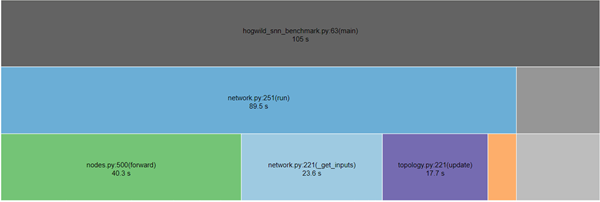
\includegraphics[width=\linewidth]{cprofile.png}
\caption{Results from running cProfile on a single-threaded SNN implementation.}
\label{fig_sim}
\end{figure}

Given these results, we focused on modifying the algorithm so that the layer, synapse and weight updates could be performed in parallel using multiple threads. The initial approach taken utilized Python's \verb|Thread| class. 

\begin{algorithm}
\caption{Multithreaded SNN Pseudocode}
\begin{algorithmic}
%
\FOR{$t=0$ \TO num\_timesteps}
\FOR{$l=0$ \TO num\_layers} do layer[l].forward()
\ENDFOR
\FOR{$c=0$ \TO num\_connections}
\ENDFOR
\FOR{$c=0$ \TO num\_connections}
\ENDFOR
\ENDFOR
\end{algorithmic}
\end{algorithm}

\subsection{Experimental Procedure} 





\section{Results}
% Note that the IEEE does not put floats in the very first column
% - or typically anywhere on the first page for that matter. Also,
% in-text middle ("here") positioning is typically not used, but it
% is allowed and encouraged for Computer Society conferences (but
% not Computer Society journals). Most IEEE journals/conferences use
% top floats exclusively. 
% Note that, LaTeX2e, unlike IEEE journals/conferences, places
% footnotes above bottom floats. This can be corrected via the
% \fnbelowfloat command of the stfloats package.


\subsection{CNN Results}
\textbf{Figure 5} and \textbf{Figure 6} illustrate the results collected from the multithreaded CNN executed on both CPU and GPU systems respectively. While the multithreading did provide improvements, it fell short of utilizing the architecture's full potential. In \textbf{Figure 5}, it can be seen that for all three executions, the peak throughput is reached at about 20 threads. After, as thread count increases, the throughput began to decreased. The greatest throughput measured is when the batch size is 128 at 507 ops/s. For this batch size, the throughput at one thread is 252 ops/s. This translates to a speedup of about 2. Using Amdahl's law, it is calculated that, at this CNN's implementations best, the percentage of instructions being parallelized is about 52.5\%. 
\par
In both \textbf{Figure 5} and \text{Figure 6}, it can be seen that the CNN execution with the batch size of 64 clearly output performs the execution with batch size of 32. A similar but less significant 

\begin{figure}[!t]
\centering
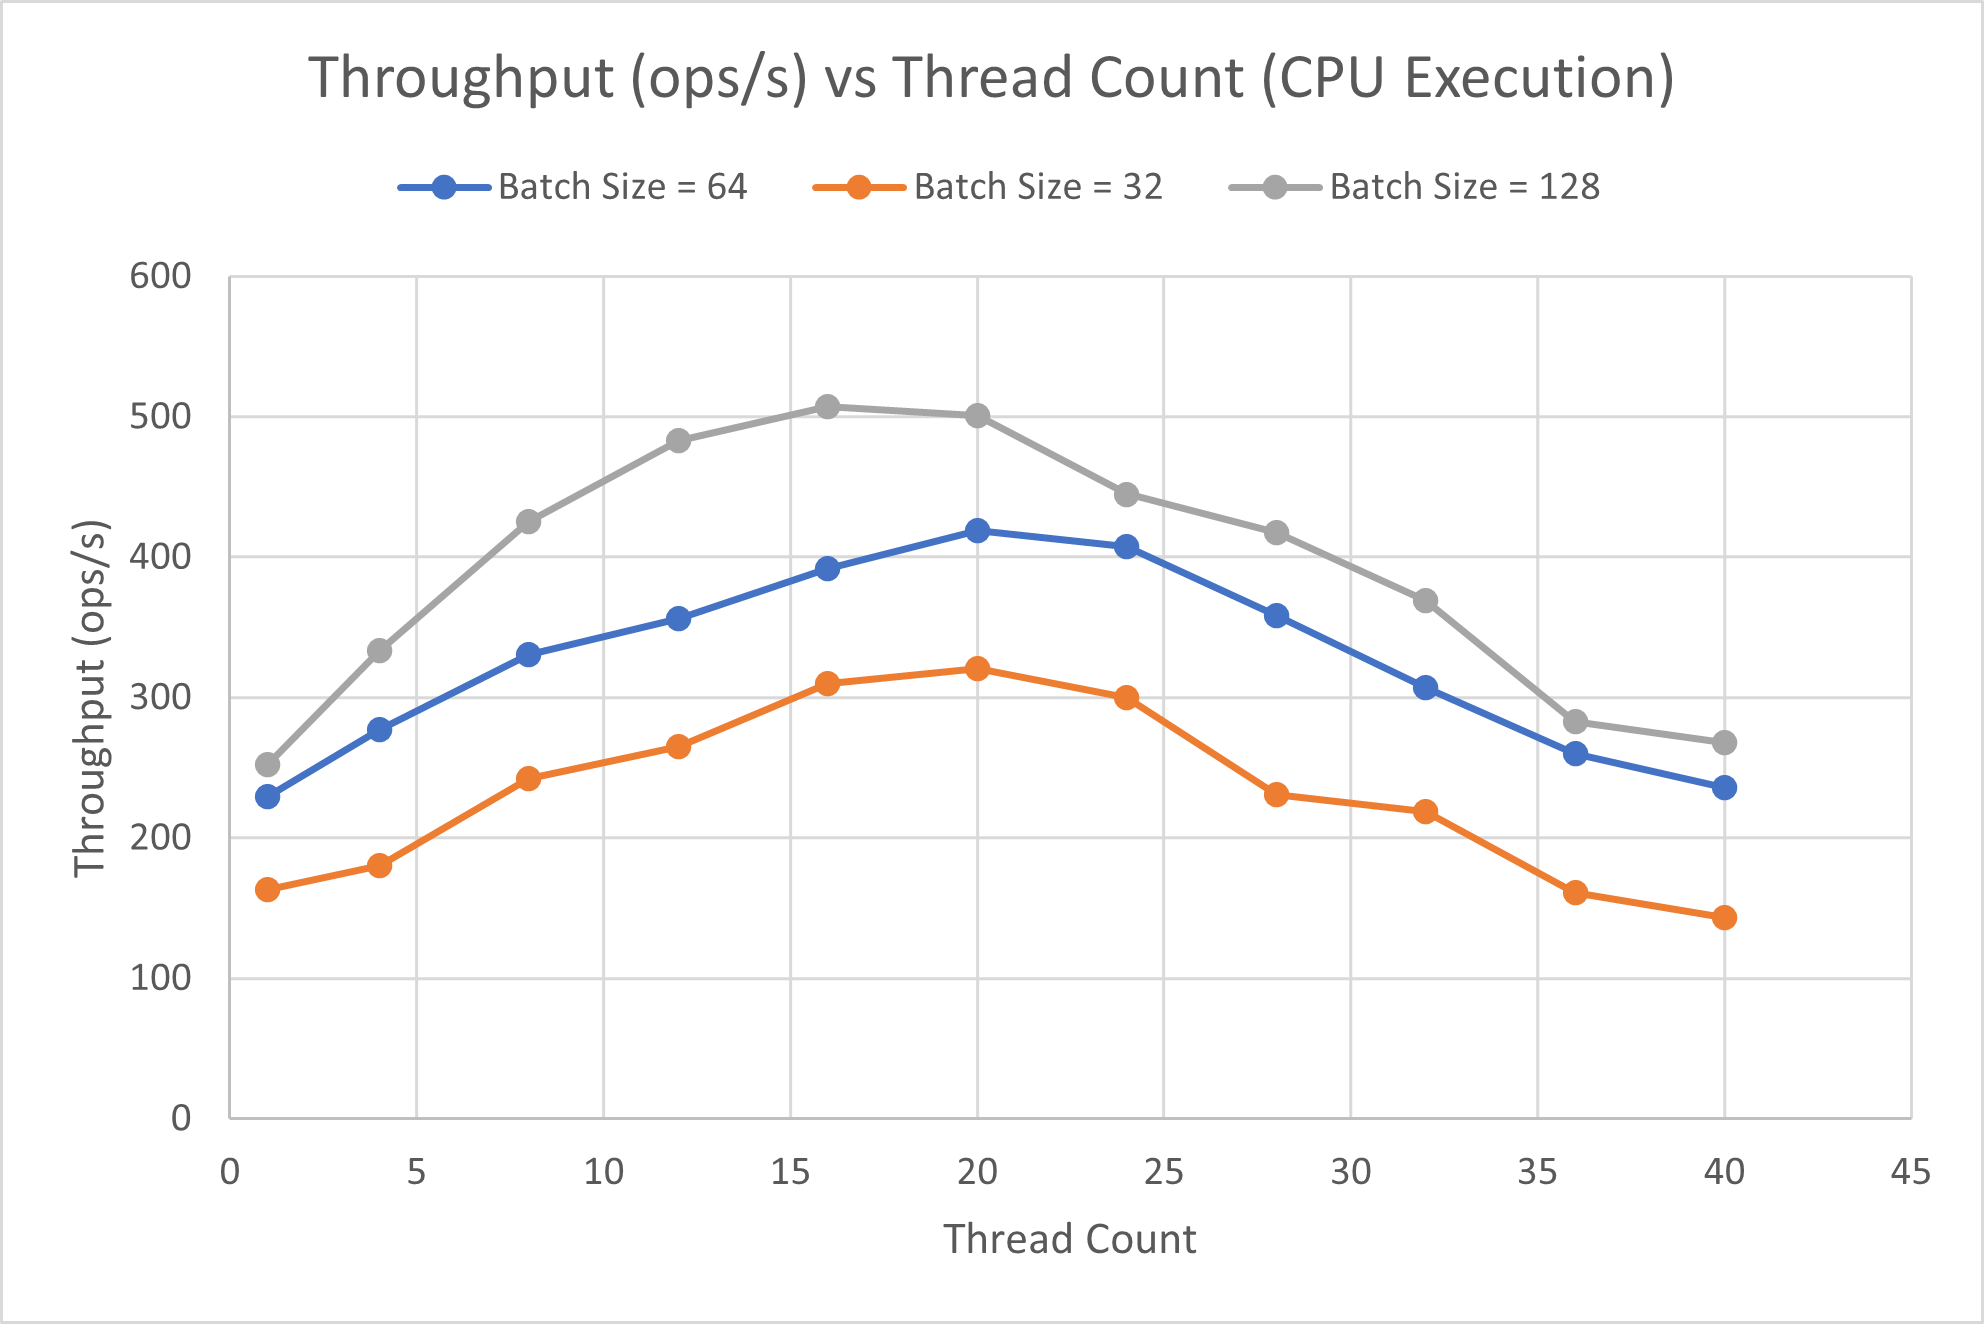
\includegraphics[width=\linewidth]{CNN_CPU_Throughput.png}
\caption{Results from running the CNN Variations on the CPU}
\label{fig_sim}
\end{figure}

\begin{figure}[!t]
\centering
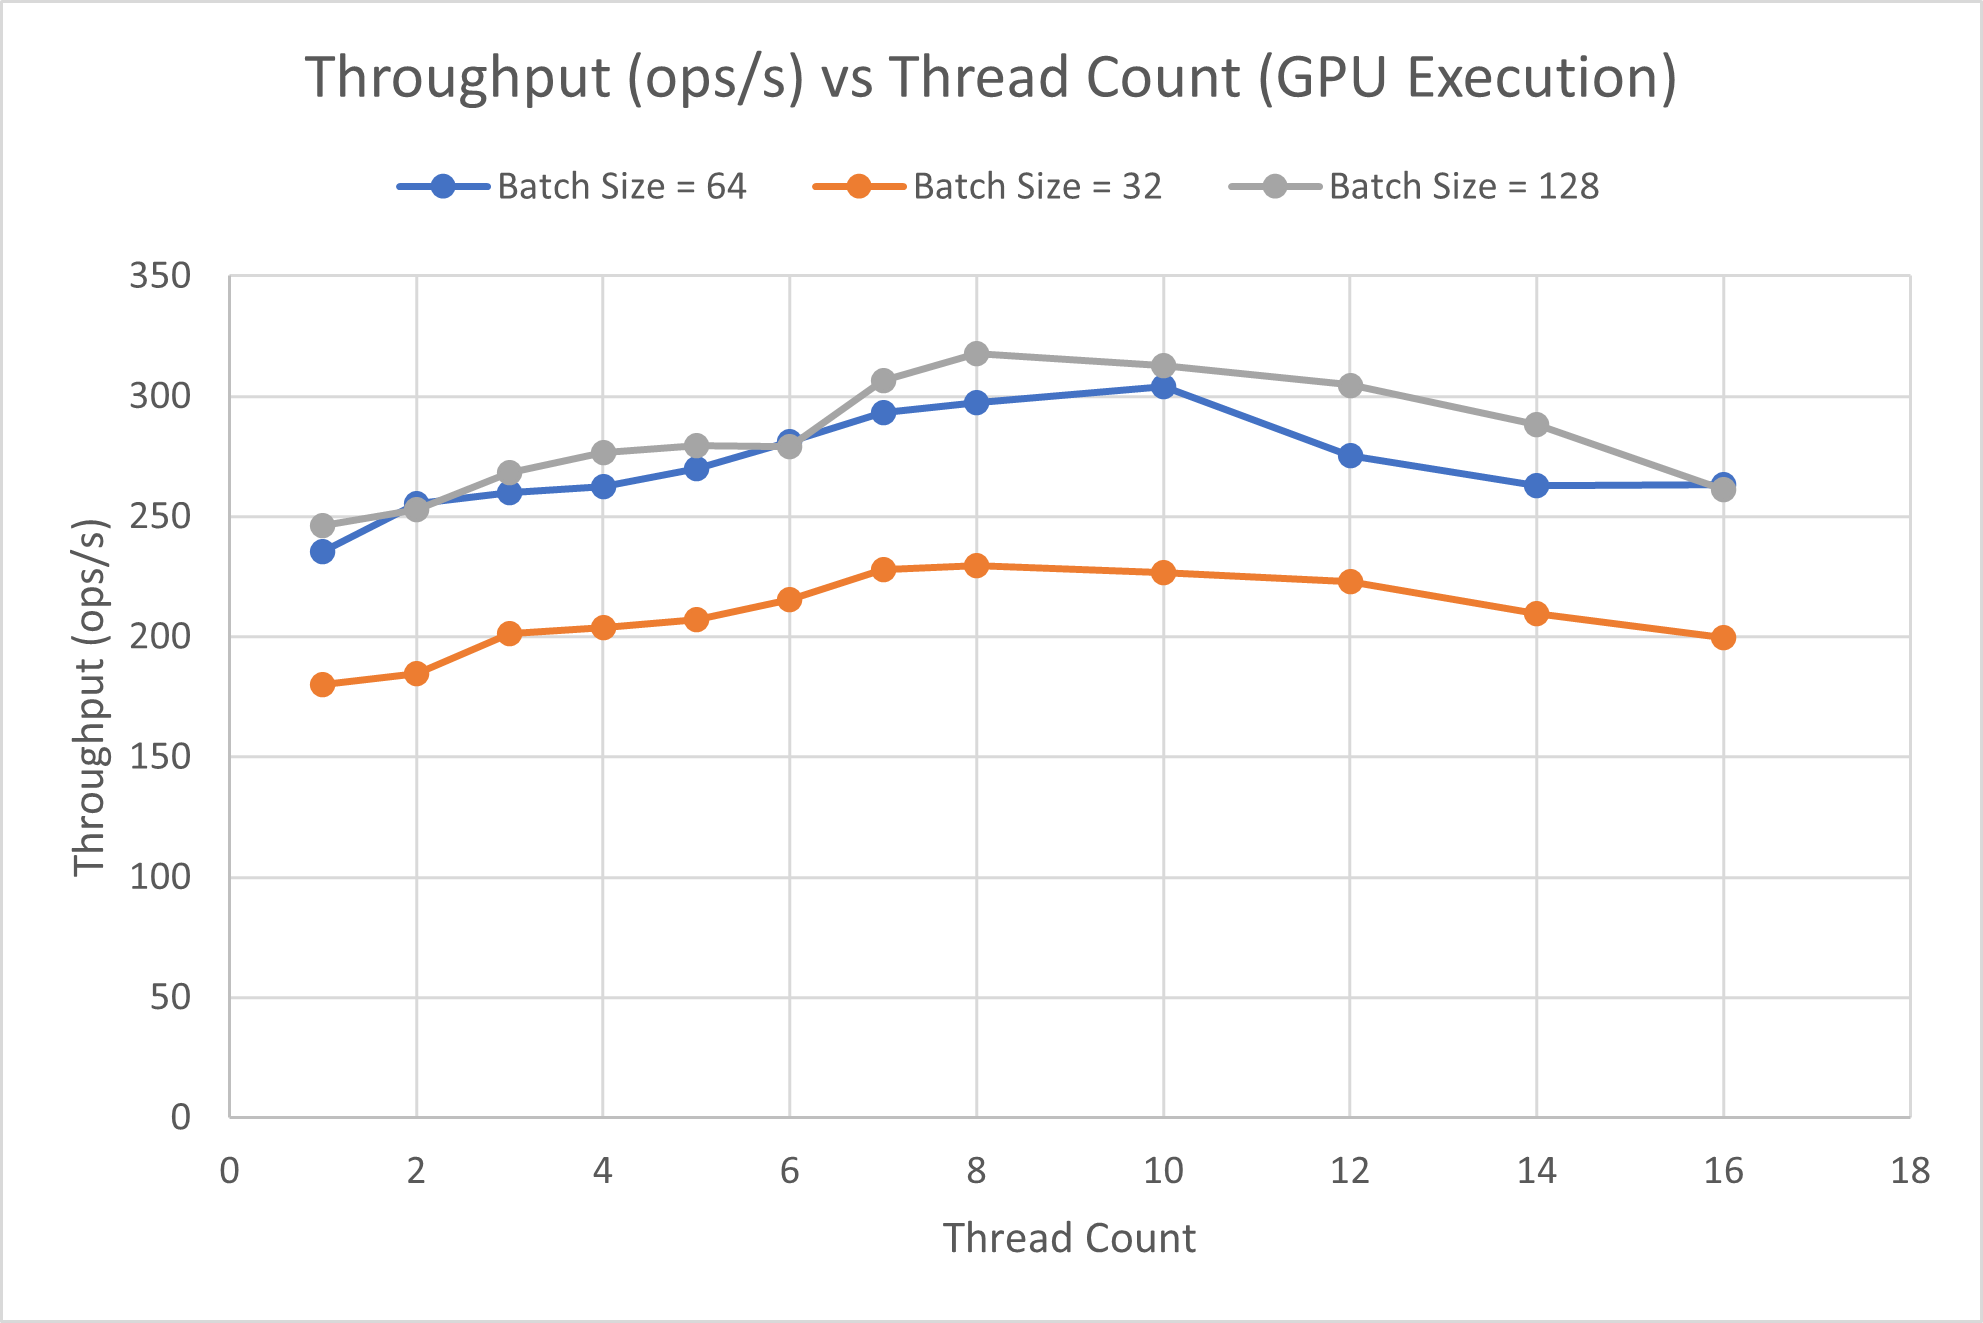
\includegraphics[width=\linewidth]{CNN_GPU_Throughput.png}
\caption{Results from running the CNN Variations on the GPU}
\label{fig_sim}
\end{figure}



\subsection{SNN Results}


\begin{figure}[!t]
\centering
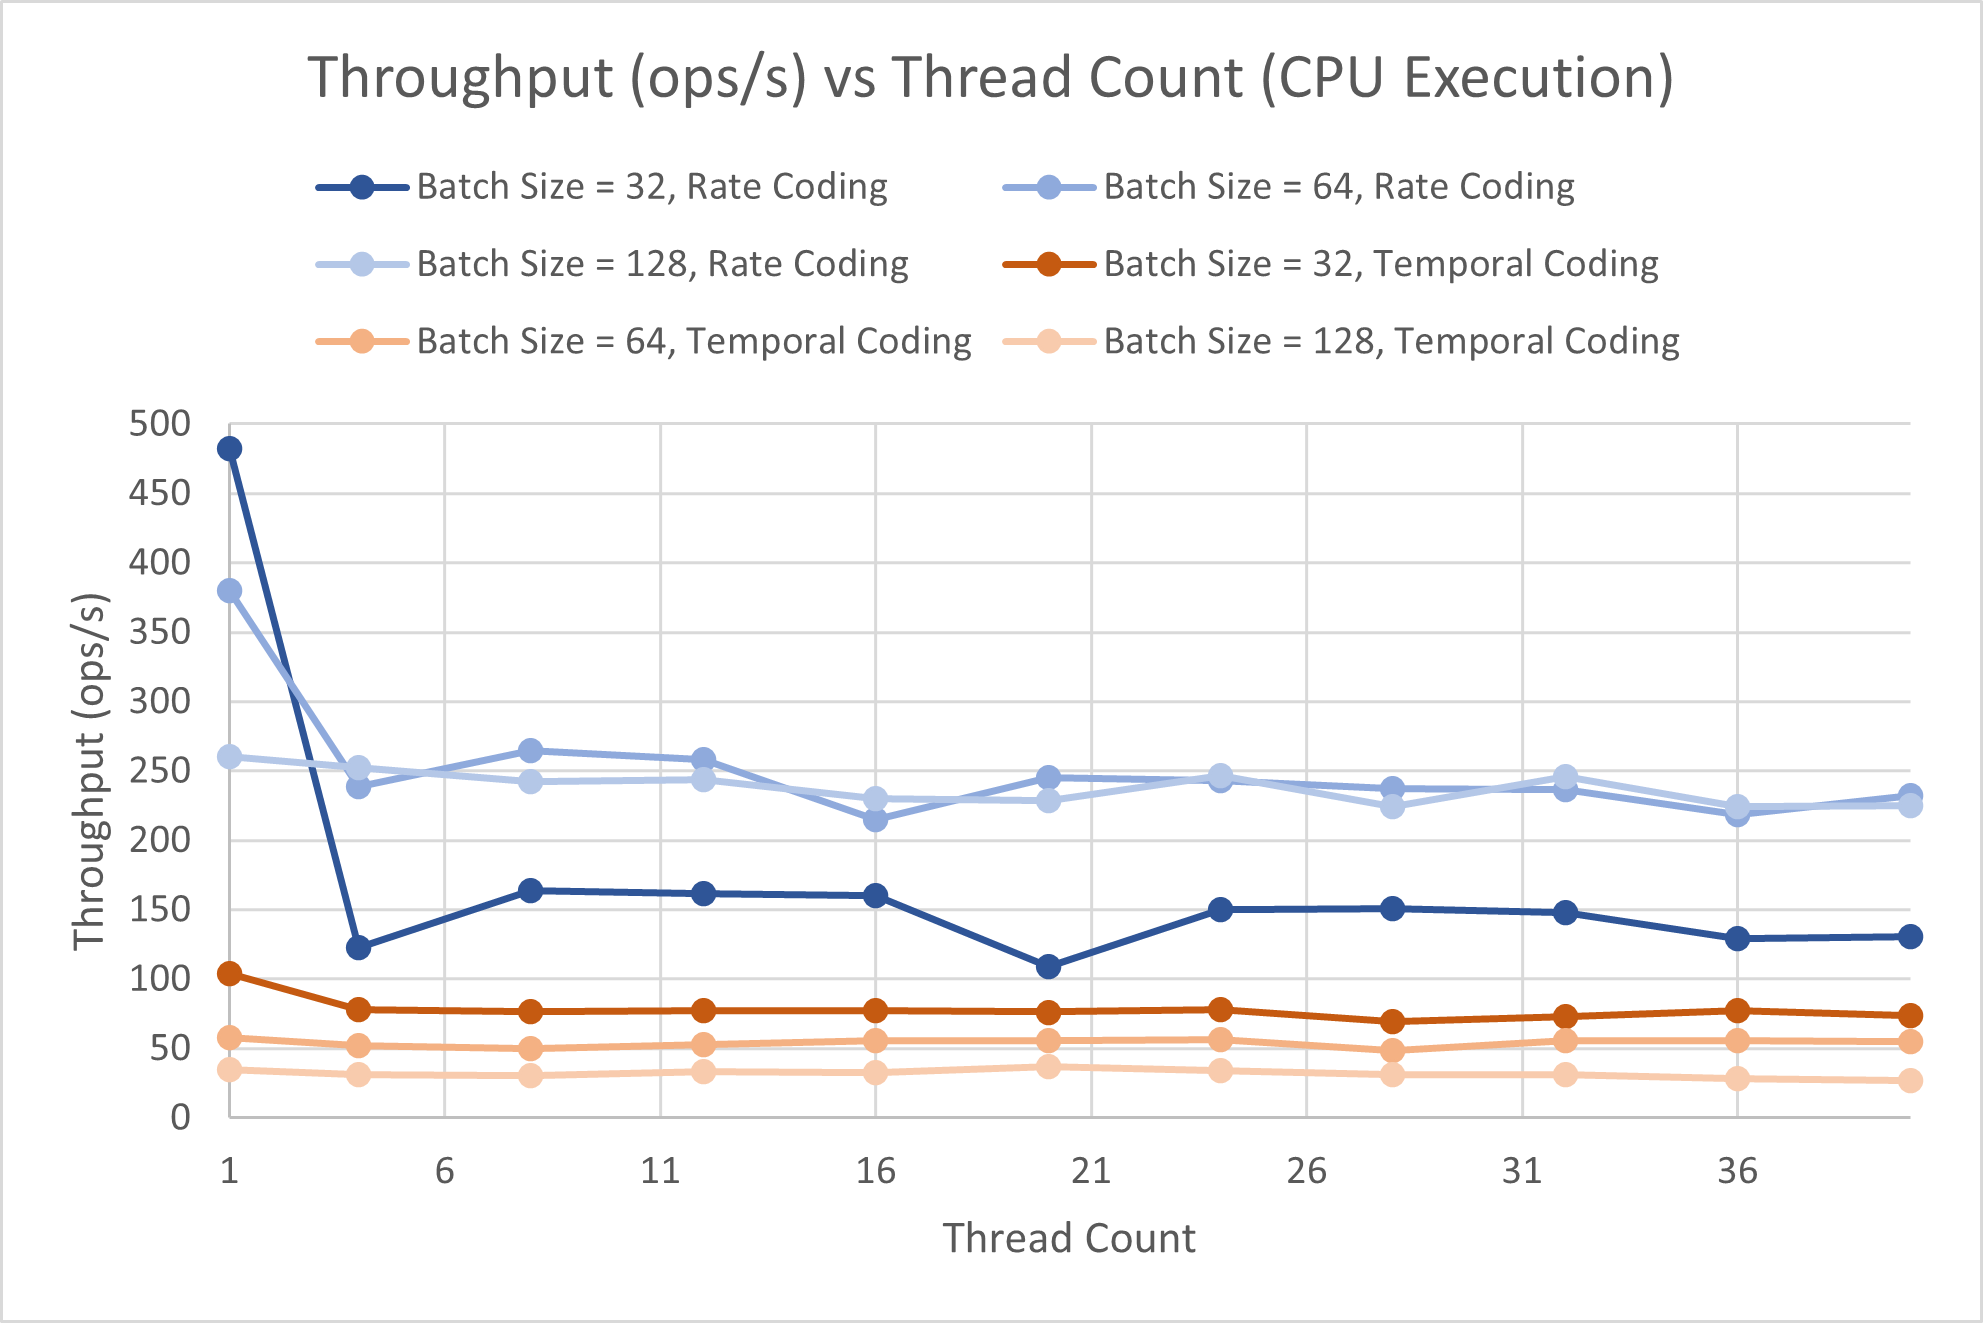
\includegraphics[width=\linewidth]{snn_results1.png}
\caption{Results from running the SNN Variations on the CPU}
\label{fig_sim}
\end{figure}

\begin{figure}[!t]
\centering
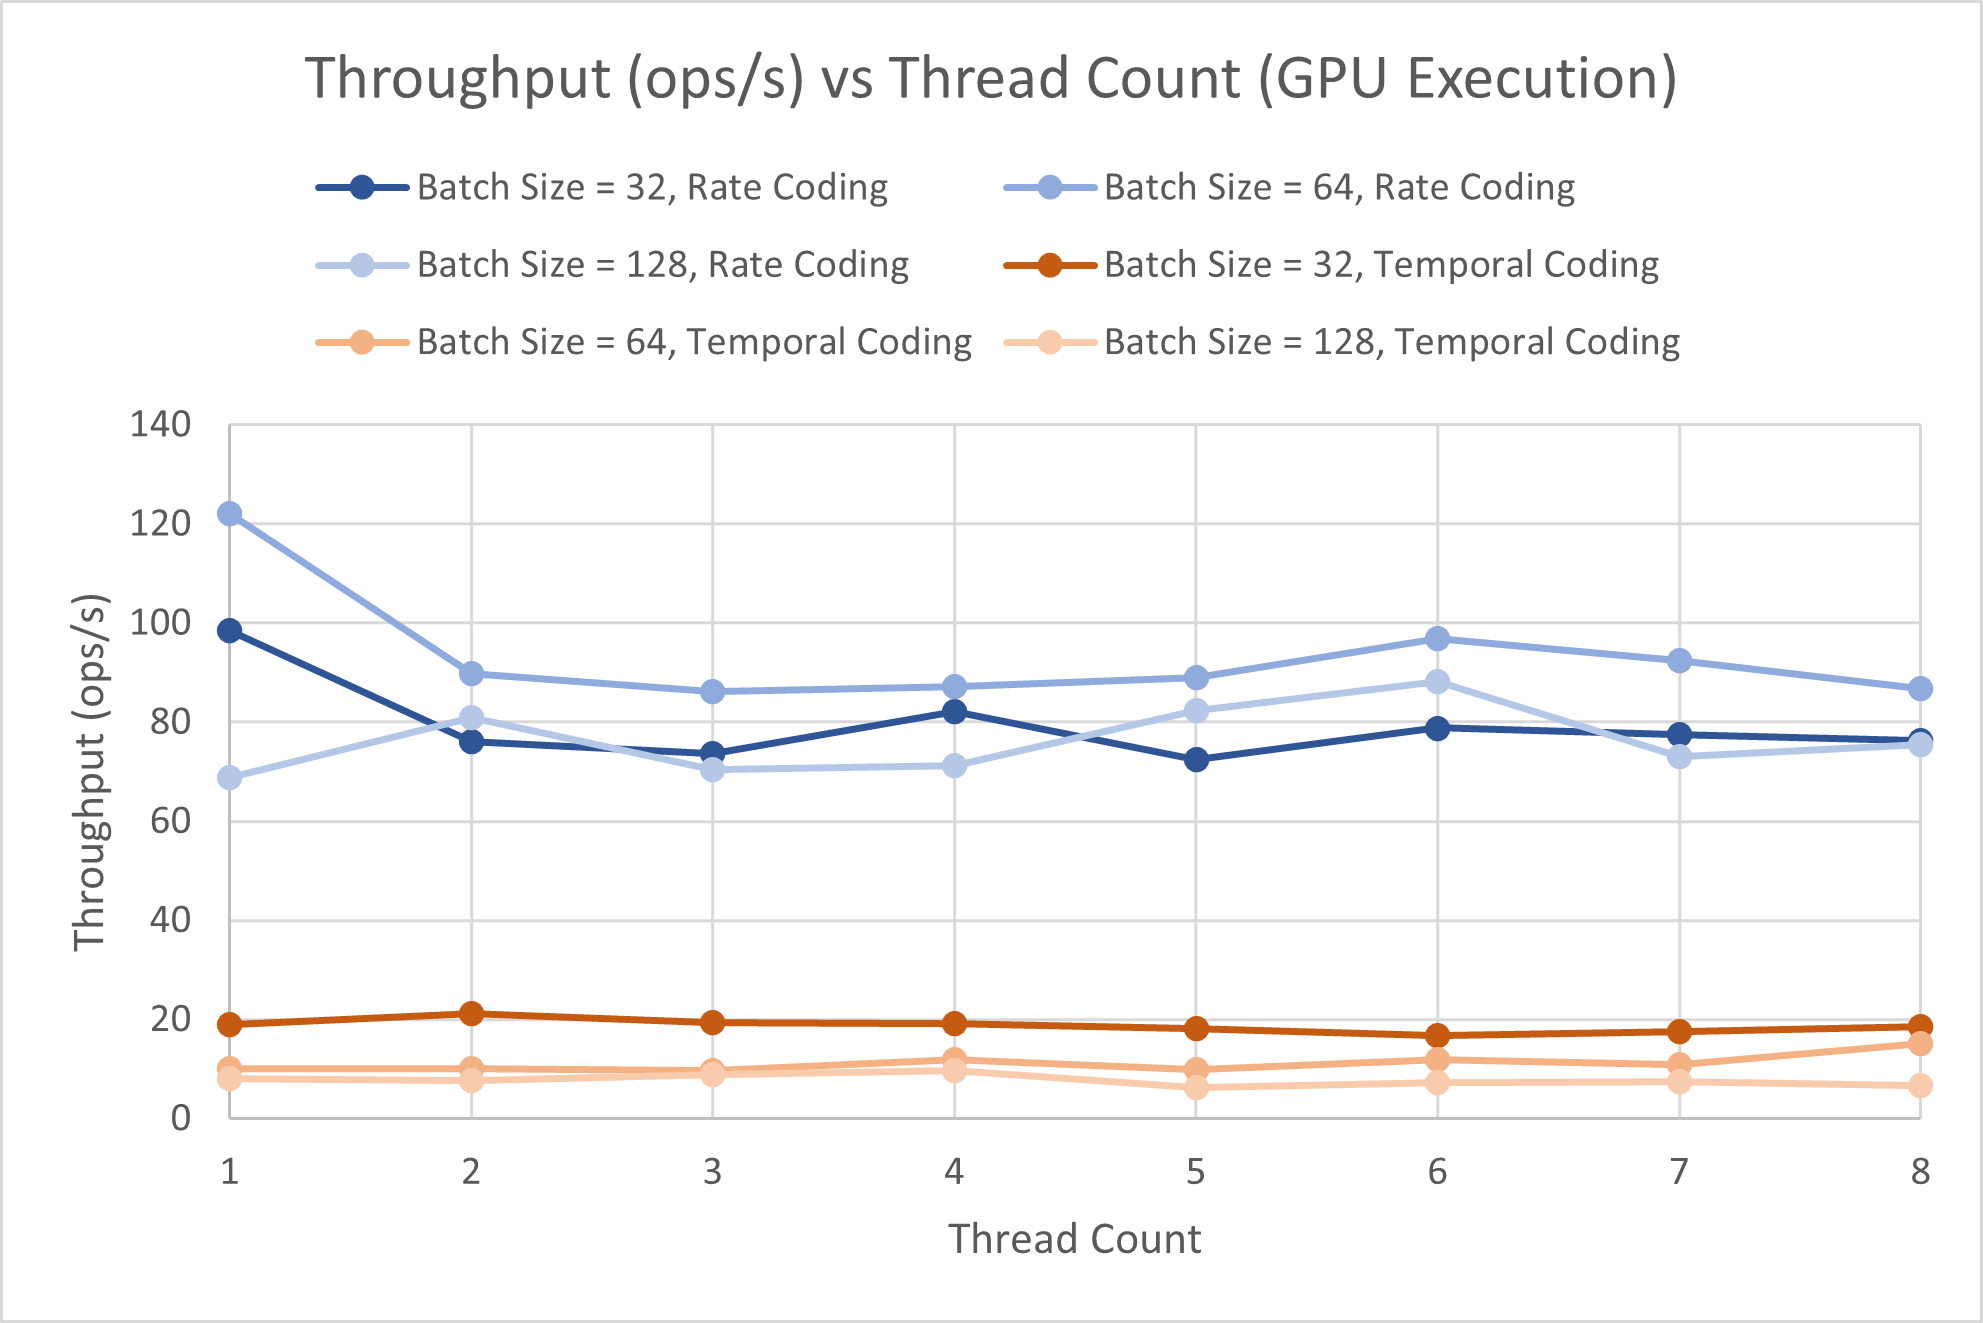
\includegraphics[width=\linewidth]{snn_results2.png}
\caption{Results from running the SNN Variations on the GPU}
\label{fig_sim}
\end{figure}

\textbf{Figure 8} and \textbf{Figure 9} show the results from running the multithreaded SNN algorithm on the CPU and GPU systems respectively. As seen in each of the figures, adding threads to perform layer, synapse and weight updates substantially decreased the throughput of the system. On the CPU-based system, the best multithreaded execution is approximately 50\% slower than the single threaded execution. Similarly, on the GPU-based system, the best multithreaded execution is approximately 20\% slower than the single threaded execution.


\subsection{Multithreaded Analysis}

We investigate the reason for this decrease in throughput by individually timing the threads instantiated by the \verb|ThreadPool| object. \textbf{Figure 9} shows the results of measuring (1) the average time it takes for a thread to get its job from the pool, (2) the average time it takes for a thread to execute this task, and (3) the average amount of time it takes for all tasks to complete. These measurements were recorded for the layer update and weight update tasks. It can be observed that the initialization of a thread takes up nearly 50\% of the execution time for both layer and weight updates. We suspect that because Python is a higher level scripting language, the multithreading features of the language have not been well optimized. Python further does not allow users to specify the priority of threads. Using a lower level programming language such as C or C++ may be able to improve the performance here by reducing the time it takes for threads to receive their tasks. 

Additionally, threads initialized in the multithreaded algorithm take a longer amount of time to perform their task than the single threaded version. We believe that the policy employed by the scheduler is partially the reason for this, since worker threads may compete with other processing running on the system. To further understand this issue, we analyzed the start and end times of threads performing layer updates as shown in \textbf{Figure 10}. The results of this experiment show all of the threads begin processing their layer updates at approximately the same time. However, the time at which a given thread completes its update occurs later if the thread was initialized at a later time (i.e., a higher thread index). At this time we cannot conclude why this behavior was observed, but we suspect that it is again, scheduler related. 

\begin{figure}[!t]
\centering
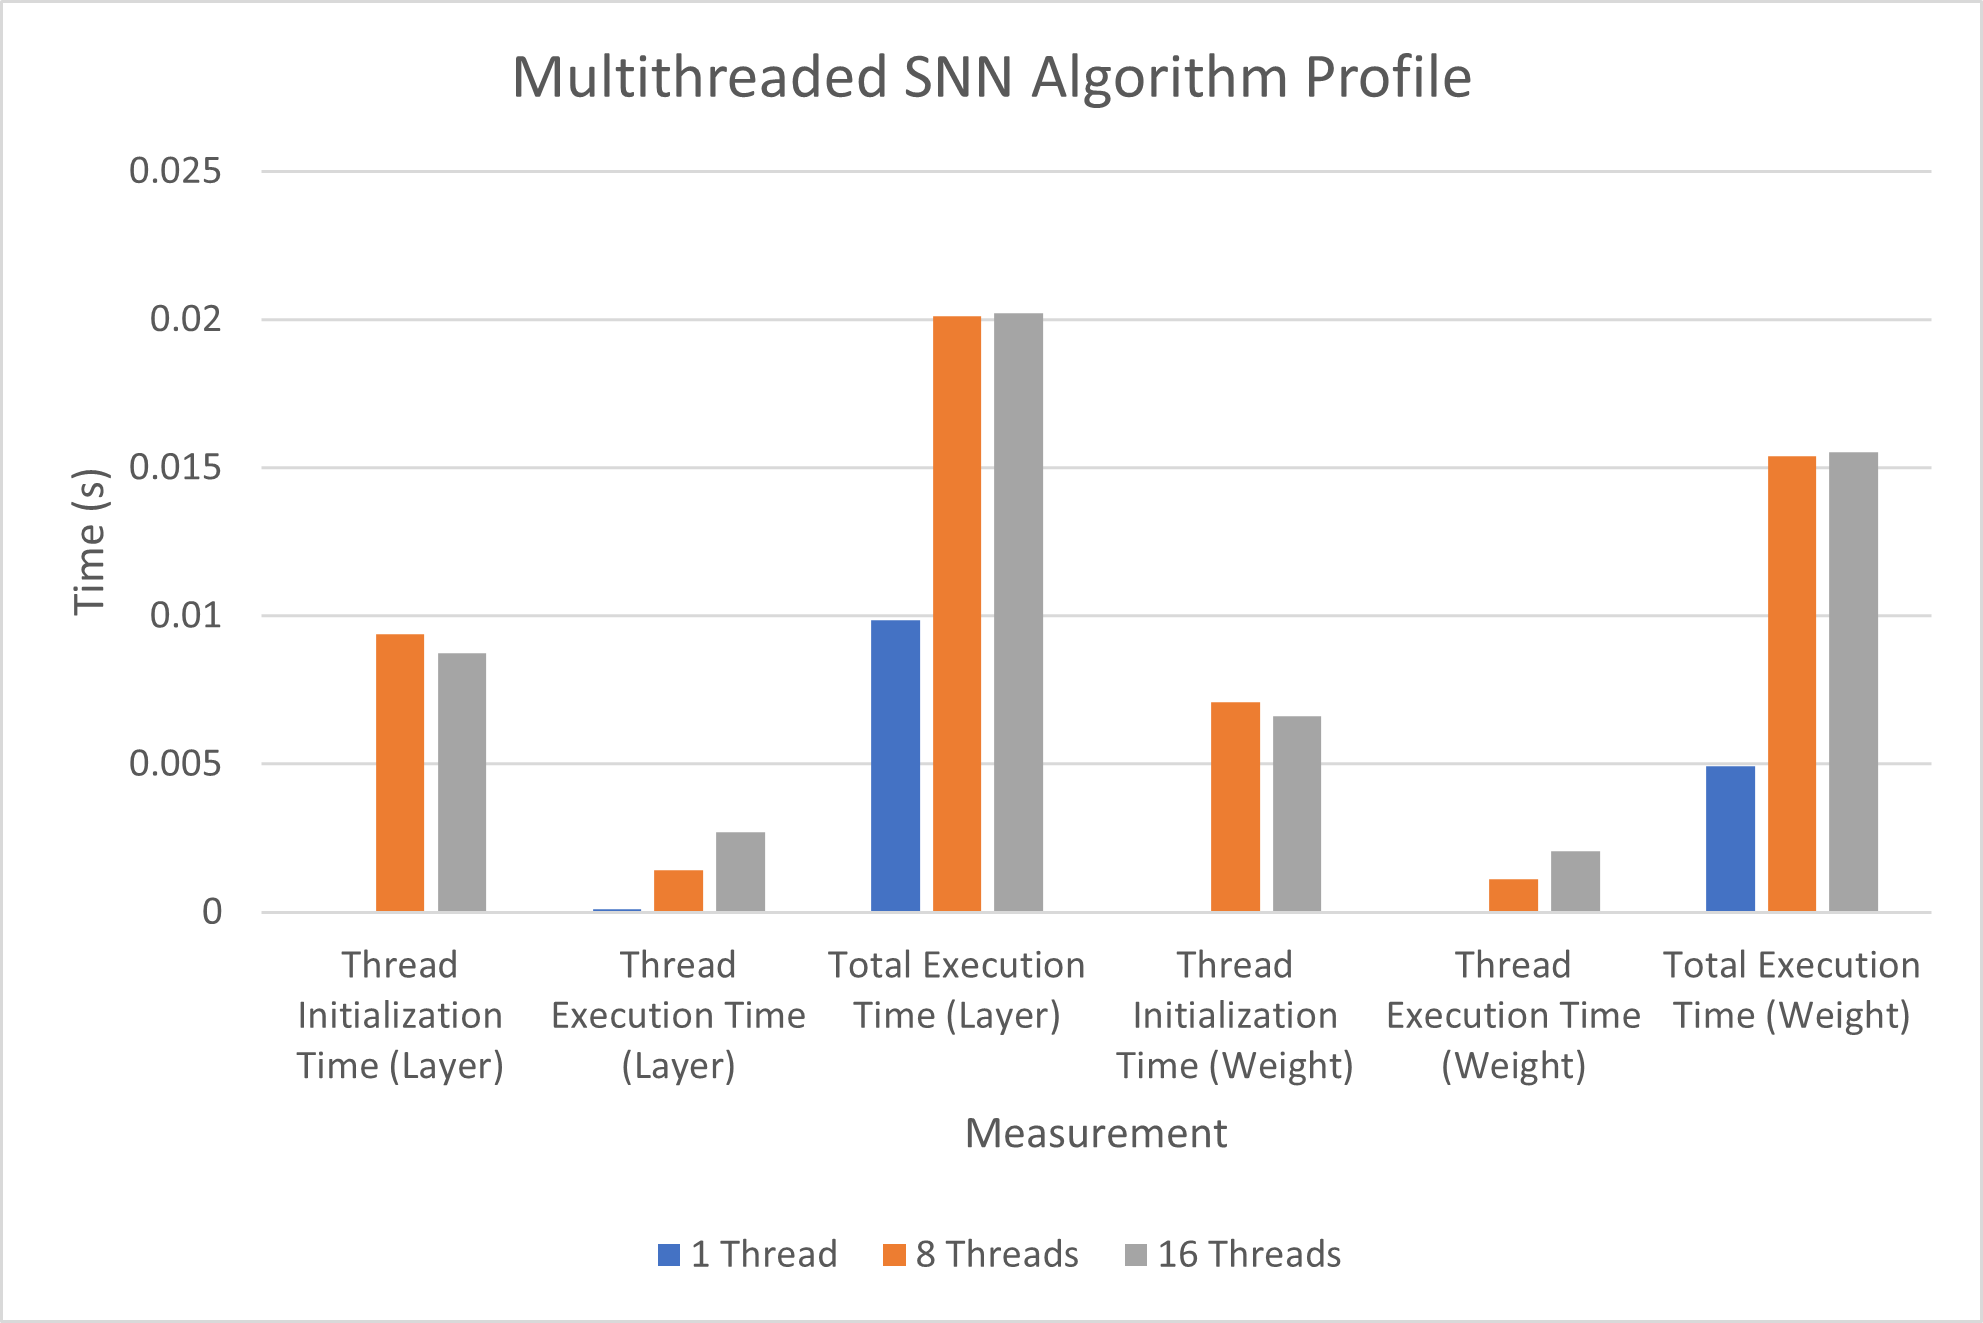
\includegraphics[width=\linewidth]{thread_profile.png}
\caption{Results from benchmarking ThreadPool tasks (Layer Updates and Weight Updates)}
\label{fig_sim}
\end{figure}

\begin{figure}[!t]
\centering
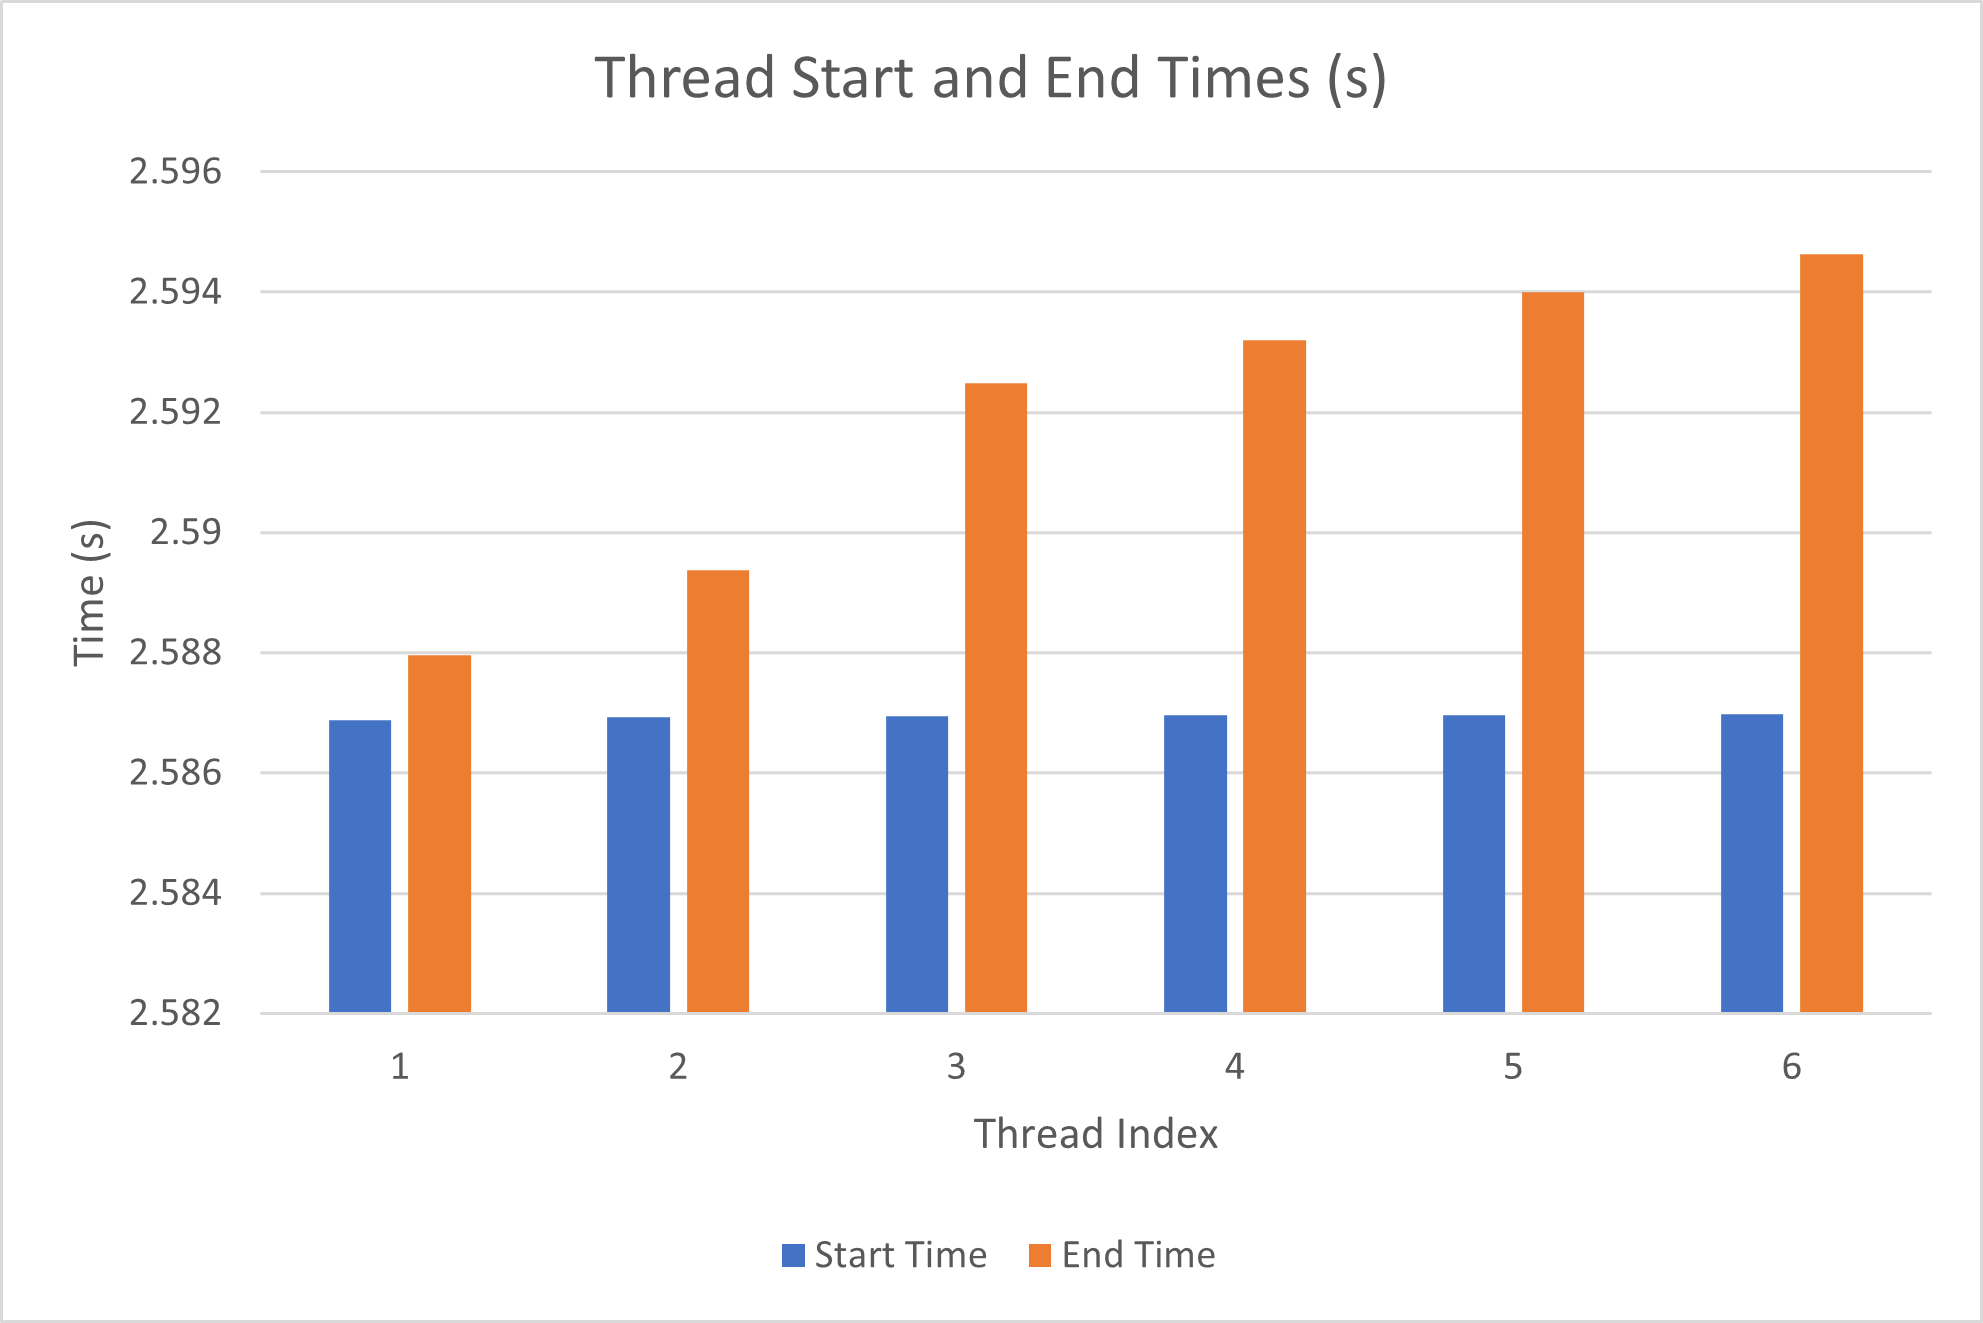
\includegraphics[width=\linewidth]{thread_start_times.png}
\caption{Results from measuring ThreadPool task start and end times (Layer Updates)}
\label{fig_sim}
\end{figure}


\section{Conclusion and Future Work}
The conclusion goes here.





% if have a single appendix:
%\appendix[Proof of the Zonklar Equations]
% or
%\appendix  % for no appendix heading
% do not use \section anymore after \appendix, only \section*
% is possibly needed

% use appendices with more than one appendix
% then use \section to start each appendix
% you must declare a \section before using any
% \subsection or using \label (\appendices by itself
% starts a section numbered zero.)
%



% trigger a \newpage just before the given reference
% number - used to balance the columns on the last page
% adjust value as needed - may need to be readjusted if
% the document is modified later
%\IEEEtriggeratref{8}
% The "triggered" command can be changed if desired:
%\IEEEtriggercmd{\enlargethispage{-5in}}

% references section

% can use a bibliography generated by BibTeX as a .bbl file
% BibTeX documentation can be easily obtained at:
% http://mirror.ctan.org/biblio/bibtex/contrib/doc/
% The IEEEtran BibTeX style support page is at:
% http://www.michaelshell.org/tex/ieeetran/bibtex/
%\bibliographystyle{IEEEtran}
% argument is your BibTeX string definitions and bibliography database(s)
%\bibliography{IEEEabrv,../bib/paper}
%
% <OR> manually copy in the resultant .bbl file
% set second argument of \begin to the number of references
% (used to reserve space for the reference number labels box)

%%%%%%%%%%%%%%%%%%%%%%%%%%%%%%%%%%%%%%%%%% REFERENCES %%%%%%%%%%%%%%%%%%%%%%%%%%%%%%%%%%%%%%%%%%%%%%%%%%%%%%%%%%%%%%%%%%%
\bibliographystyle{IEEEtran}
\bibliography{IEEEabrv,database.bib}

%%%%%%%%%%%%%%%%%%%%%%%%%%%%%%%%%%%%%%%%%%%%%%%%%%%%%%%%%%%%%%%%%%%%%%%%%%%%%%%%%%%%%%%%%%%%%%%%%%%%%%%%%%%%%%%%%%%%%%%%%

% biography section
% 
% If you have an EPS/PDF photo (graphicx package needed) extra braces are
% needed around the contents of the optional argument to biography to prevent
% the LaTeX parser from getting confused when it sees the complicated
% \includegraphics command within an optional argument. (You could create
% your own custom macro containing the \includegraphics command to make things
% simpler here.)
%\begin{IEEEbiography}[{\includegraphics[width=1in,height=1.25in,clip,keepaspectratio]{mshell}}]{Michael Shell}
% or if you just want to reserve a space for a photo:

% \begin{IEEEbiography}{Michael Shell}
% Biography text here.
% \end{IEEEbiography}

% % if you will not have a photo at all:
% \begin{IEEEbiographynophoto}{John Doe}
% Biography text here.
% \end{IEEEbiographynophoto}

% insert where needed to balance the two columns on the last page with
% biographies
%\newpage

% \begin{IEEEbiographynophoto}{Jane Doe}
% Biography text here.
% \end{IEEEbiographynophoto}

% You can push biographies down or up by placing
% a \vfill before or after them. The appropriate
% use of \vfill depends on what kind of text is
% on the last page and whether or not the columns
% are being equalized.

%\vfill

% Can be used to pull up biographies so that the bottom of the last one
% is flush with the other column.
%\enlargethispage{-5in}



% that's all folks
\end{document}


